%%%%%%%%%%%%%%%%%%%%%%%%%%%%%%%%%%%%%%%%%%%%%%%%%%%%%%%%%%%%%%%%%%%%%%%%%%%%%%%%%%%%%%%%%%%%%%%%%%%
%
% Copyright (c) 2015 Rodrigo A. Melo <rmelo@inti.gob.ar>
% Copyright (c) 2015 Bruno Valinoti  <valinoti@inti.gob.ar>
% Copyright (c) 2015 Leandro Tozzi   <ltozzi@inti.gob.ar>
% Copyright (c) 2015 Instituto Nacional de Tecnología Industrial
%
%%%%%%%%%%%%%%%%%%%%%%%%%%%%%%%%%%%%%%%%%%%%%%%%%%%%%%%%%%%%%%%%%%%%%%%%%%%%%%%%%%%%%%%%%%%%%%%%%%%

\documentclass[conference]{../../resources/IEEEtran/IEEEtran}
\usepackage[utf8]{inputenc}   % El texto de entrada es utf8
\usepackage[T1]{fontenc}      % Codificación de las fonts
%\usepackage[spanish]{babel}   % Selección de español
%\selectlanguage{spanish}
\usepackage{graphicx,subfigure,listings}
%\usepackage{tikz,tikz-timing}
\usepackage[keeplastbox]{flushend}

%%%%%%%%%%%%%%%%%%%%%%%%%%%%%%%%%%%%%%%%%%%%%%%%%%%%%%%%%%%%%%%%%%%%%%%%%%%%%%%%%%%%%%%%%%%%%%%%%%%

\title{Analog Front End Design of Contactless Smart Card for Standard ISO14443A}

\author{
  \IEEEauthorblockN{Flavio Galimberti, Agust\'in Grosso, Yao-Ming Kuo, Juan T\'antera}
  \IEEEauthorblockA{Universidad Tecnol\'ogica Nacional\\
  Facultad Regional Buenos Aires\\
  Email: \{ykuo, agrosso\}@frba.utn.edu.ar, \{fgalimberti, juantantera\}@est.frba.utn.edu.ar}
  %\thanks{}
%  \IEEEauthorblockN{Blinded}
%  \IEEEauthorblockA{Blinded}
}

%Para que aparezca thanks
%\IEEEoverridecommandlockouts

%Aquí se corrige mala separación en silabas
%\hyphenation{e-jem-plo}

\begin{document}

%\ninept % Si queremos letra más chica (para que entre más texto).

% Frequently used
\newcommand {\backward}                {{\it backward}}
\newcommand {\bit}                     {{\it bit}}
\newcommand {\bits}                    {{\it bits}}
\newcommand {\buffer}                  {{\it buffer}}
\newcommand {\bus}                     {{\it bus}}
\newcommand {\byte}                    {{\it byte}}
\newcommand {\bytes}                   {{\it bytes}}
\newcommand {\clock}                   {{\it clock}}
\newcommand {\constraints}             {{\it constraints}}
\newcommand {\core}                    {{\it core}}
\newcommand {\cores}                   {{\it cores}}
\newcommand {\default}                 {{\it default}}
\newcommand {\dimmer}                  {{\it dimmer}}
\newcommand {\dipsw}                   {{\it dip-switch}}
\newcommand {\driver}                  {{\it driver}}
\newcommand {\ff}                      {{\it flip-flop}}
\newcommand {\forward}                 {{\it forward}}
\newcommand {\frames}                  {{\it frames}}
\newcommand {\fw}                      {{\it firmware}}
\newcommand {\gbt}                     {{\it Giga Bit Transceiver}}
\newcommand {\generic}                 {{\it generic}}
\newcommand {\generics}                {{\it generics}}
\newcommand {\hw}                      {{\it hardware}}
\newcommand {\kit}                     {{\it kit}}
\newcommand {\kits}                    {{\it kits}}
\newcommand {\led}                     {{\it led}}
\newcommand {\leds}                    {{\it leds}}
\newcommand {\lfsr}                    {{\it Linear Feedback Shift Register}}
\newcommand {\make}                    {{\it make}}
\newcommand {\Makefile}                {{\it Makefile}}
\newcommand {\master}                  {{\it master}}
\newcommand {\masters}                 {{\it masters}}
\newcommand {\offset}                  {{\it offset}}
\newcommand {\overflow}                {{\it overflow}}
\newcommand {\pipeline}                {{\it pipeline}}
\newcommand {\reset}                   {{\it reset}}
\newcommand {\resize}                  {{\it resize}}
\newcommand {\runtime}                 {{\it runtime}}
\newcommand {\script}                  {{\it script}}
\newcommand {\slave}                   {{\it slave}}
\newcommand {\slaves}                  {{\it slaves}}
\newcommand {\snippet}                 {{\it snippet}}
\newcommand {\sw}                      {{\it software}}
\newcommand {\switch}                  {{\it switch}}
\newcommand {\tarball}                 {{\it tarball}}
\newcommand {\tb}                      {{\it testbench}}
\newcommand {\timer}                   {{\it timer}}
\newcommand {\variables}               {{\it variables}}
\newcommand {\word}                    {{\it word}}
\newcommand {\words}                   {{\it words}}

% FFT related
\newcommand {\butterflies}             {{\it butterflies}}
\newcommand {\butterfly}               {{\it butterfly}}
\newcommand {\dft}                     {{\it Discrete Fourier Transform}}
\newcommand {\dif}                     {{\it Decimation In Frequency}}
\newcommand {\dit}                     {{\it Decimation In Time}}
\newcommand {\fft}                     {{\it Fast Fourier Transform}}
\newcommand {\rdxc}                    {{\it Radix-4}}
\newcommand {\rdxd}                    {{\it Radix-2}}
\newcommand {\tfr}                     {{\it twiddle factors}}

% Comunication Related
\newcommand {\broadcast}               {{\it broadcast}}
\newcommand {\isdbt}                   {{\it Integrated Services Digital Broadcasting Terrestial}}
\newcommand {\ofdm}                    {{\it Orthogonal Frequency Division Multiplexing}}

% Dali related
\newcommand {\dali}                    {{\it Digital Addressable Lighting Interface}}
\newcommand {\dmx}                     {{\it Digital MultipleX}}
\newcommand {\dsi}                     {{\it Digital Signal Interface}}

%MIPS related
\newcommand {\MIPS}		       {{\it Microprocessor without Interlocked Pipeline Stages}}
\newcommand {\RISC}		       {{\it Reduced Instruction Set Computer}}


\maketitle

%%%%%%%%%%%%%%%%%%%%%%%%%%%%%%%%%%%%%%%%%%%%%%%%%%%%%%%%%%%%%%%%%%%%%%%%%%%%%%%%%%%%%%%%%%%%%%%%%%%

\begin{abstract}
This paper describes a set of analog front end design for contactless smart cards which complies with ISO 14443-2 Type A. It has been implemented in Globalfoundries 130nm (GF130) CMOS process. The design and implementation was manufactured by MOSIS through the Educational Program. The analog front end operates at 13.56MHz with data rate 106kbps. This paper will show the simulation using Synopsys HSPICE and the corresponding test for the CMOS process GF130.
\end{abstract}

\begin{IEEEkeywords}
CMOS technology  Analog integrated circuits, Rectifiers, Transceivers, Amplitude shift keying, Modulation, Demodulation, Regulators, Clocks, Power conditioning, RFID tags, Smart cards
\end{IEEEkeywords}

%%%%%%%%%%%%%%%%%%%%%%%%%%%%%%%%%%%%%%%%%%%%%%%%%%%%%%%%%%%%%%%%%%%%%%%%%%%%%%%%%%%%%%%%%%%%%%%%%%%

\section{Introduction}
\label{sec:intro}
In recent years, Radio Frequency Identification systems (RFID) \cite{rfid_handbook} have become very popular in many service industries, purchasing and distribution logistics, industry, manufacturing companies and material flow systems. In contrast to earlier techniques like barcodes, RFID is more favored because of its longer operation distance, higher precision, faster processing speed and storage capabilities. RFID makes it possible to identify objects and store data in a single silicon chip. This paper studies the RF circuits design proposal of contactless IC card meeting ISO/IEC14443-2 \cite{nfc_spec} standard and validates topologies testing the IC. This design meets the performance request with the designed circuits, and has been successfully implemented with 130nm CMOS technology.

%%%%%%%%%%%%%%%%%%%%%%%%%%%%%%%%%%%%%%%%%%%%%%%%%%%%%%%%%%%%%%%%%%%%%%%%%%%%%%%%%%%%%%%%%%%%%%%%%%%

\section{ISO/IEC14443-2}
\label{sec:iso}
\subsection{Types of RF interface}
In ISO/IEC 14443-2 describes two types of RF interface about contactless IC cards which operate at 13.56 MHz: Type A and Type B. 

In Type A, the signal from PCD (Proximity Coupling Device) to PICC (Proximity Integrated Circuit Device) is modulated in ASK (Amplitude Shift Keying) with modulation index 100\%. When receiving the data from PCD, the PICC can’t process the data because the absence of the clock source. 

In Type B,  the signal from PCD to PICC is defined to be modulated with BPSK by carrier, and the signal from PCD to PICC is modulated in ASK with modulation index 10\%, which make it possible for PICC to work continuously. Therefore, the solution given by Type B could reach higher data rate, but the design of the circuits would be more complicated. The ASK index 10\% is harder to detect than index 100\%.

This paper describes the circuit design for the Type A. 


\subsection{Analog Front-End Modules}

The contactless IC card contains two main sections: RF section and Data Processing Unit (DPU). The modules in RF section are demonstrated in Fig.\ref{fig:modules}, which comprises Power Supply Generator (PSG), Clock Generator (CG), Voltage Regulator (VR), Power On Reset (POR), Modulator  and Demodulator. 

\begin{figure}[]
  \centering
  \includegraphics[page=9,width=80mm]{images-crop.pdf}
  \caption{Contactless IC card modules}
  \label{fig:modules}
\end{figure}

When the PICC enters to the RF field, the signal coupled by antenna can generate power supply through PSG. The PSG consists of a rectifier and a Shunt Regulator. The VG regulates the power of PSG and gives a constant voltage to the rest of the modules. As soon as the power supply reaches the operating condition, the POR gives a low level signal to reset all the Flip-Flops of the DPU. The modulator and demodulator are modules that let the PCD communicate with PICC.

%%%%%%%%%%%%%%%%%%%%%%%%%%%%%%%%%%%%%%%%%%%%%%%%%%%%%%%%%%%%%%%%%%%%%%%%%%%%%%%%%%%%%%%%%%%%%%%%%%%

\section{IC Circuit Design}
\label{sec:design}
The previous section demonstrates the RF modules that involve  the communication between PCD and PICC. This section will describe in detail each module of the analog front-end for ISO/IEC 14443A (see Fig. \ref{fig:afe}).

\begin{figure}[]
  \centering
  \includegraphics[page=10,width=80mm]{images-crop.pdf}
  \caption{PICC Analog Front-end}
  \label{fig:afe}
\end{figure}

\subsection{Power Supply Generator (PSG)}

The Power Supply Generator splits into two parts: signal rectification and power limitation.

The first part rectifies the RF field signal to get power supply for the chip, a full NMOS bridge rectifier \cite{rfid_rect1}\cite{rfid_rect2} was implemented in this design. And the second part consists of a Shunt resistor. The Shunt resistor is capable to limit the voltage of the antenna and protects the whole chip. ISO/IEC14443-2 requires the PICC to work when magnetic intensity between 1.5-7.5A/m rms. Therefore the PICC must work in these extreme conditions.  

The simplified schematic of signal rectification is shown in Fig. \ref{fig:rect} and power limitation (Shunt resistor) is shown in Fig. \ref{fig:shunt}.

\begin{figure}[h]
  \centering
  \includegraphics[page=11,width=60mm]{images-crop.pdf}
  \caption{Full Wave Rectifier}
  \label{fig:rect}
\end{figure}

\begin{figure}[h]
  \centering
  \includegraphics[page=12,width=60mm]{images-crop.pdf}
  \caption{Shunt Resistor}
  \label{fig:shunt}
\end{figure}

\subsection{Clock Generator (CG)}

The Clock Generator recovers the clock from the antenna and is used by the DPU. This module generates a clock source of 13.56 MHz. Basically consists of two FF/D (clock divider by 2) and a XOR logic gate. 

The difference of phase between RF+ and RF- are 180 degrees, it is easy to take advantage of this property to recompose the clock. The simplified schematic is shown in Fig. \ref{fig:clk} and the simulation in the Fig. \ref{fig:clk_sim}.

A frequency divider by 4 is placed at the output of the clock generator, reducing the work frequency also reduces the power consumed. On the other hand, Carrier-Frequency/4 (3.39MHz) is used for the DPU, because the FDT (Frame Delay Time)  defined in ISO/IEC14443-3 is for all commands are divisor of this frequency.
 

\begin{figure}[]
  \centering
  \includegraphics[page=13,width=60mm]{images-crop.pdf}
  \caption{Clock Generator schematic}
  \label{fig:clk}
\end{figure}

\begin{figure}[]
  \centering
  \includegraphics[page=14,width=80mm]{images-crop.pdf}
  \caption{Clock recovery simulation}
  \label{fig:clk_sim}
\end{figure}

\subsection{Voltage Regulator (VR)}

The Voltage Regulator \cite{rfid_ldo} regulates the voltage supplied from PSG and provide a constant DC voltage at the output of this module. The VR is known as the series pass regulator, as shown in Fig. \ref{fig:ldo}. It consists of 3 major parts. Operational amplifier (OP-AMP) is used as error amplifier. A series pass transistor forms a current amplifier. R1 and R2 are used as resistive voltage divider (Ecuation \ref{eq:vref}). The reference source Vref, in this case, is a beta multiplier \cite{panadero}. 

\begin{equation} \label{eq:vref}
VDD = Vref*(1+R1/R2)
\end{equation}
%$$VDD = Vref*(1+R1/R2)$$  

%Basically it consist of a reference source, in this case, a beta multiplier is used for this purpose. The OP AMP play the role of controller, it copies the reference voltage, control the variation of VRECT or VDD and reflects the reference voltage to the output.

\begin{figure}[]
  \centering
  \includegraphics[page=15,width=60mm]{images-crop.pdf}
  \caption{Voltage Regulator schematic}
  \label{fig:ldo}
\end{figure}

\subsection{Modulator}

The modulator \cite{rfid_modulador} transmits the signal from PICC to PCD. There are two different types of load modulation: resistive and capacitive modulation. Both types create a subcarrier next to 13.56MHz. The NMOS are switched on and off in time with the encoded data. This will vary the load (resistive) or resonance frequency  (capacitive) of the transponder.  Resistive modulation was adopted in this design for its simplicity. The schematic is shown in Fig. \ref{fig:mod}.

\begin{figure}[h]
  \centering
  \includegraphics[page=16,width=40mm]{images-crop.pdf}
  \caption{Modulator schematic}
  \label{fig:mod}
\end{figure}

\subsection{Demodulator}

The demodulator recovers the digital signals from the ASK signal transmitted from PCD. An Envelope Extractor (EE) \cite{rfid_demodulador} is needed to extract the data. The digital signal is recovered by connecting the output of the EE with the input of the buffer. The circuit is shown in Fig. \ref{fig:demod}. 

\begin{figure}[h]
  \centering
  \includegraphics[page=17,width=80mm]{images-crop.pdf}
  \caption{Demdulator schematic}
  \label{fig:demod}
\end{figure}

\subsection{Power On Reset (POR)}

The Power On Reset module is used to reset the digital machine and put it into idle state. It consists of a RC low pass network. When the chip enter to the RF field, the VR turns on and power all the modules. The POR module holds the voltage of the VR and delays it. This signal applies to the reset pin of the Flip-Flops in the digital machine. The schematic is demonstrated in Fig. \ref{fig:por}. 

\begin{figure}[h]
  \centering
  \includegraphics[page=18,width=20mm]{images-crop.pdf}
  \caption{POR schematic}
  \label{fig:por}
\end{figure}

%%%%%%%%%%%%%%%%%%%%%%%%%%%%%%%%%%%%%%%%%%%%%%%%%%%%%%%%%%%%%%%%%%%%%%%%%%%%%%%%%%%%%%%%%%%%%%%%%%%

\section{IC Circuit Floorplaning}
\label{sec:floor}
The corresponding layout \cite{dali_man} is shown in Fig. \ref{fig:layout}, it was designed for two different CMOS processes: Global Foundries 130nm and On Semiconductor 500nm, but the topologies are similar. The analog Front End covers 0.3mm x 0.2mm in 130nm (Fig. \ref{fig:layout}.a) and 0.6mm x 0.5mm in 500nm (Fig. \ref{fig:layout}.b).

The design of GF130 was shipped by MOSIS, it is shown in Fig. \ref{fig:layout}.c. 

\begin{figure}[h]
  \centering
  \includegraphics[page=19,width=80mm]{images-crop.pdf}
  \caption{(a) ONC5 Layout, (b) GF130 Layout, (c) GF130 Chip}
  \label{fig:layout}
\end{figure}

%%%%%%%%%%%%%%%%%%%%%%%%%%%%%%%%%%%%%%%%%%%%%%%%%%%%%%%%%%%%%%%%%%%%%%%%%%%%%%%%%%%%%%%%%%%%%%%%%%%

\section{Measurement \& Validation}
\label{sec:valid}
In order to verify and validate the design, each module are tested and compared with simulation results. The corresponding tests verifies the feasibility of the design.

The measurement of the clock generator and a phase of the RF field (RF+) is shown in the Fig. \ref{fig:meas}.a. The wave demonstrates that the CG works well and can divide the clock 13.56MHz/4. The ripple of the clock is due to the noise of external power source that the ring pad is connected. 

The Fig. \ref{fig:meas}.b shows the comparison between RF+ with the output of the POR module. It can be seen the delay of the POR in relation to the input signal.

\begin{figure}[h]
  \centering
  \includegraphics[page=20,width=80mm]{images-crop.pdf}
  \caption{(a) Clk/4 vs RF+, (b) RF+ vs Power On Reset, (c) Clk/4 vs Demodulator}
  \label{fig:meas}
\end{figure}

%%%%%%%%%%%%%%%%%%%%%%%%%%%%%%%%%%%%%%%%%%%%%%%%%%%%%%%%%%%%%%%%%%%%%%%%%%%%%%%%%%%%%%%%%%%%%%%%%%%

\section{Conclusion}
\label{sec:conclusion}
An analog front-end circuit for ISO/IEC14443A compatible RFID transponder IC was designed and implemented by using the Global Foundries 130nm (eight-metal/mim-capacitor) and On Semiconductor 500 nm (three-metal/two-poly) CMOS process. The measurement demonstrated that the transponder IC works properly (converts RF power to DC voltage, extracts the clock and data, and correctly sends data back). Using GF130 could reduce drastically the area in comparison with ONC5. This is a huge improvement compared with the existing products.

%%%%%%%%%%%%%%%%%%%%%%%%%%%%%%%%%%%%%%%%%%%%%%%%%%%%%%%%%%%%%%%%%%%%%%%%%%%%%%%%%%%%%%%%%%%%%%%%%%%

\section{Acknowledgements}
\label{sec:ack}
The authors would like to thank to Nanolab - UTN FRBA for their contributions and support and to the Centro de Micro y Nano Electronica del Bicentenario (CMNB-INTI) for the use of the testing facilities. 
We also thank MOSIS and Synopsys academic programs.
The integrated circuit was designed using Synopsys \cite{synopsys} tools under the Synopsys University Program. The chips were fabricated through the MOSIS foundry service supported by the MOSIS Educational Program (MEP).

%%%%%%%%%%%%%%%%%%%%%%%%%%%%%%%%%%%%%%%%%%%%%%%%%%%%%%%%%%%%%%%%%%%%%%%%%%%%%%%%%%%%%%%%%%%%%%%%%%%

%%%%%%%%%%%%%%%%%%%%%%%%%%%%%%%%%%%%%%%%%%%%%%%%%%%%%%%%%%%%%%%%%%%%%%%%%%%%%%%%%%%%%%%%%%%%%%%%%%%





%\IEEEtriggeratref{11}
%\footnotesize

\bibliographystyle{../../resources/IEEEtranBST2/IEEEtran}
\bibliography{../../resources/IEEEtranBST2/IEEEabrv,../shared,nfc}

%%%%%%%%%%%%%%%%%%%%%%%%%%%%%%%%%%%%%%%%%%%%%%%%%%%%%%%%%%%%%%%%%%%%%%%%%%%%%%%%%%%%%%%%%%%%%%%%%%%

\end{document}
